% This is samplepaper.tex, a sample chapter demonstrating the
% LLNCS macro package for Springer Computer Science proceedings;
% Version 2.20 of 2017/10/04
%
\documentclass[runningheads]{llncs}
%
\usepackage{graphicx}
\usepackage{listings}
\usepackage[T1]{fontenc}
\usepackage[portuguese]{babel}
\usepackage{hyphenat}
\hyphenation{mate-mática recu-perar}
\usepackage{xcolor}
\usepackage{amsmath}
\usepackage{hyperref}

\definecolor{codegreen}{rgb}{0,0.6,0}
\definecolor{codegray}{rgb}{0.5,0.5,0.5}
\definecolor{codepurple}{rgb}{0.58,0,0.82}
\definecolor{backcolour}{rgb}{0.95,0.95,0.92}

\lstdefinestyle{mystyle}{
    backgroundcolor=\color{backcolour},   
    commentstyle=\color{codegreen},
    keywordstyle=\color{magenta},
    numberstyle=\tiny\color{codegray},
    stringstyle=\color{codepurple},
    basicstyle=\ttfamily\footnotesize,
    breakatwhitespace=false,         
    breaklines=true,                 
    captionpos=b,                    
    keepspaces=true,                 
    numbers=left,                    
    numbersep=5pt,                  
    showspaces=false,                
    showstringspaces=false,
    showtabs=false,                  
    tabsize=2
}

\lstset{style=mystyle}




\begin{document}
%

\begin{titlepage}
   \begin{center}
       \vspace*{1cm}

       \textbf{Theoretical project 1}

       \vspace{0.5cm}
        Theoretical project 1,   Mobile Robotics
            
       \vspace{1.5cm}

       \textbf{José António Filipe Santos, 98279} 
       \vfill

            
       \vspace{0.8cm}
     
       
\includegraphics[width=0.4\textwidth]{logo.jpg}
            
       Departamento de Electrónica, Telecomunicações e Informática\\
        Universidade de Aveiro\\
       Portugal\\
       May, 2023


            
   \end{center}
\end{titlepage}



\title{Theoretical project 1}
\begin{abstract}
Creation of a Extended Kalman Filter for application in a mobile robot in Matlab.
\keywords{Mobile Robotcis \and Extended Kalman Filter}
\end{abstract}
%
%
%
\section{Introduction}
This work is made with the objective of a virtual robot in an environment with multiple landmarks is 
able to localize itself using an Extended Kalman Filter. The robot is able to locate itslef in this environment 
thanks to the BeaconDetection() function. The other important function is the EKF or Exetended Kalman Filter,
with was modified to meet the requirements of the teacher.





\section{functions}
In this part of the report I will explain the functions that were created to obtain the desired results.

\subsection*{plotting\_path}
This function has two objectives, one obtainin the steps needed to reach the goal, passing through the landmarks 
and the other is to use the function in Matlab named \textbf{pchip()} to obtain the smooth path that the robot will take.

For the calculation of steps, this is based on the distance between beacons, or between the initial position and the first beacon.

The equation \begin{math}
\left(\frac{\sqrt{((x2-x1)^2+(y2-y1)^2}}{\mathrm{Dt}\, * \mathrm{Vn}}\right)
\end{math} is used to obtain the number of steps taken between beacons, where the time step and velocity.
With the number of steps aquired, we can obtain the total number of  x and y variables.
\\ 
After obtaining the total x and y values evenly spaced between the beacons, we use the \textbf{unique()} function to obtain the unique x values, 
and with these interpolated values or "xintep" values, we use the pchip function with all the beacons and the starting position, to obtain the interpolated y values. 
\\

To see the results of this function the figure \ref*{plotting_path_fig}, is showed below. 

\begin{figure}[h]
\centering
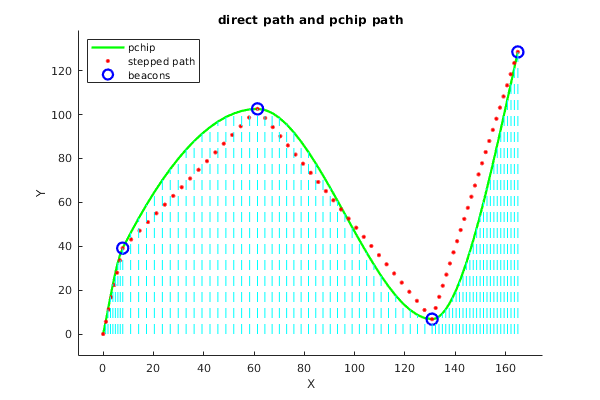
\includegraphics[width=0.9\textwidth]{plotting_path.png}
\caption{Plotting path function results}
\label{plotting_path_fig}
\end{figure}






\end{document}
